At each timestep, an appearance based probability map is generated over the observed 
RGB frame, with respect to the appearance distributions built prior to the reconstruction 
process. An example of such instantaneous map is given in Figure~\ref{figure:probobj_prob_maps}.
\begin{figure}[!htbp]
  \centering
  \begin{tabular}{cc}
    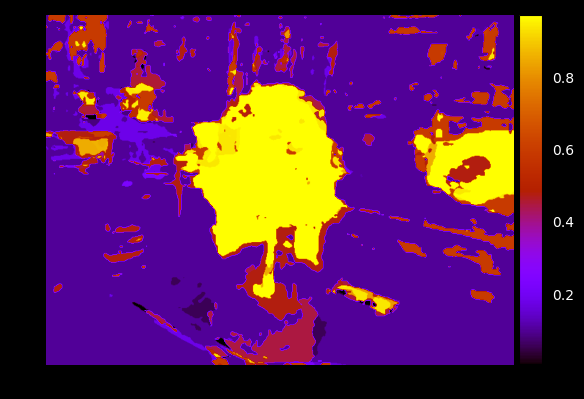
\includegraphics[width=.4\linewidth]{figures/object_recon/prob/dino.png} &
    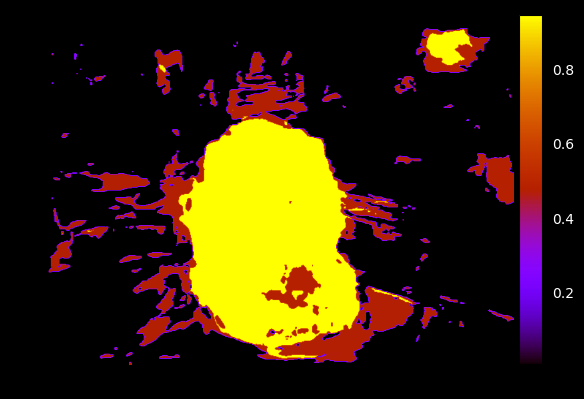
\includegraphics[width=.4\linewidth]{figures/object_recon/prob/rock.png} \\ 
    (a) & (b) \\
  \end{tabular}
  \caption[Raw Foreground Probability Maps]
  {
    \begin{tabular}[t]{@{}l@{}}
      (a) An instantaneous probability map in which much noise is present in the background.\\
      (b) A map that is very probabilistically polarized with respect to foreground and background beliefs.
    \end{tabular}
  } 
~\label{figure:probobj_prob_maps}
\end{figure}